\documentclass[titlepage]{article}
\usepackage[utf8]{inputenc}
\usepackage[left=1cm, top=0.8cm,bottom=1.2cm, textwidth=18.6cm, textheight=27cm]{geometry}
\geometry{paper=a4paper}
\usepackage{titling}
\usepackage{abstract}
\usepackage{fancyhdr}
\usepackage{amsmath}
\usepackage{gensymb}
\usepackage{graphicx}

\lhead{} \chead{} \rhead{}
\lfoot{\emph{Multimedia and computer visualisation 2015/2016}} \cfoot{} \rfoot{\thepage}
\renewcommand{\headrulewidth}{0pt}
\renewcommand{\footrulewidth}{0.4pt}
\pagestyle{fancy}


\title{Color systems conversion tool}
\author{Maciej Borkowski\\ 195968@student.pwr.edu.pl \and Michał Kowalski \\ 195447@student.pwr.edu.pl}
\date{}
\begin{document}
\maketitle

\section{Subject of project}
The goal of project was to create simple tool/application, main functionality of
which will be conversion between few, listed later, color systems. Program
should allow user to input value in one of systems, and should return result in
the rest of implemented systems. There are also two additional functionalities:
\begin{enumerate}
  \item loading a image and displaying representations of pixel under mouse
  cursor,
  \item choosing a value in some systems in graphical form, by selecting a color
  from a palette.
\end{enumerate}

% TODO cos wiecej?

\section{Color Systems}
There are many color systems, used for describing color, but they are serving
different purposes. Some of them are more precise, some are easy for humans to
describe/imagine, some are used for printing, some require less memory, and some
can describe wider range of colors.
Popular color systems include:
\begin{itemize}
  \item RGB,
  \item grayscale,
  %TODO binary,
  \item CMYK,
  \item HSV.
  %TODO YUV & YIQ
\end{itemize}
Most popular system is RGB, and most conversion algorithms are for conversions
from/to RGB. Conversions between other systems can be done by converting from
original system to RGB, and then from RGB to desired system. Those conversions
are not always perfect, because sometimes values need to be rounded, and some
color systems can't describe all colors (with grayscale being one of examples).

\subsection{RGB}
RGB (\textbf{R}ed, \textbf{G}reen, \textbf{B}lue) is most popular color system.
It is additive system, so color is created by addition of base colors (light in
one of three colors) to black (no light). Mixing max values of them is shown on
fig. \ref{fig:rgb}. Three RGB values can be described as percentage, 0-1, 0-255,
or as single hexadecimal value. 0-255 (8 bit) or hexadecimal (which is a
derivative of it) is most popular, but because it has not continous range of
values, not all colors can be perfectly described, but error is small. Main
problem with RGB system is, that result of mixing three colors is hard to
imagine for humans.

\begin{figure}[!htb]
	\centering
	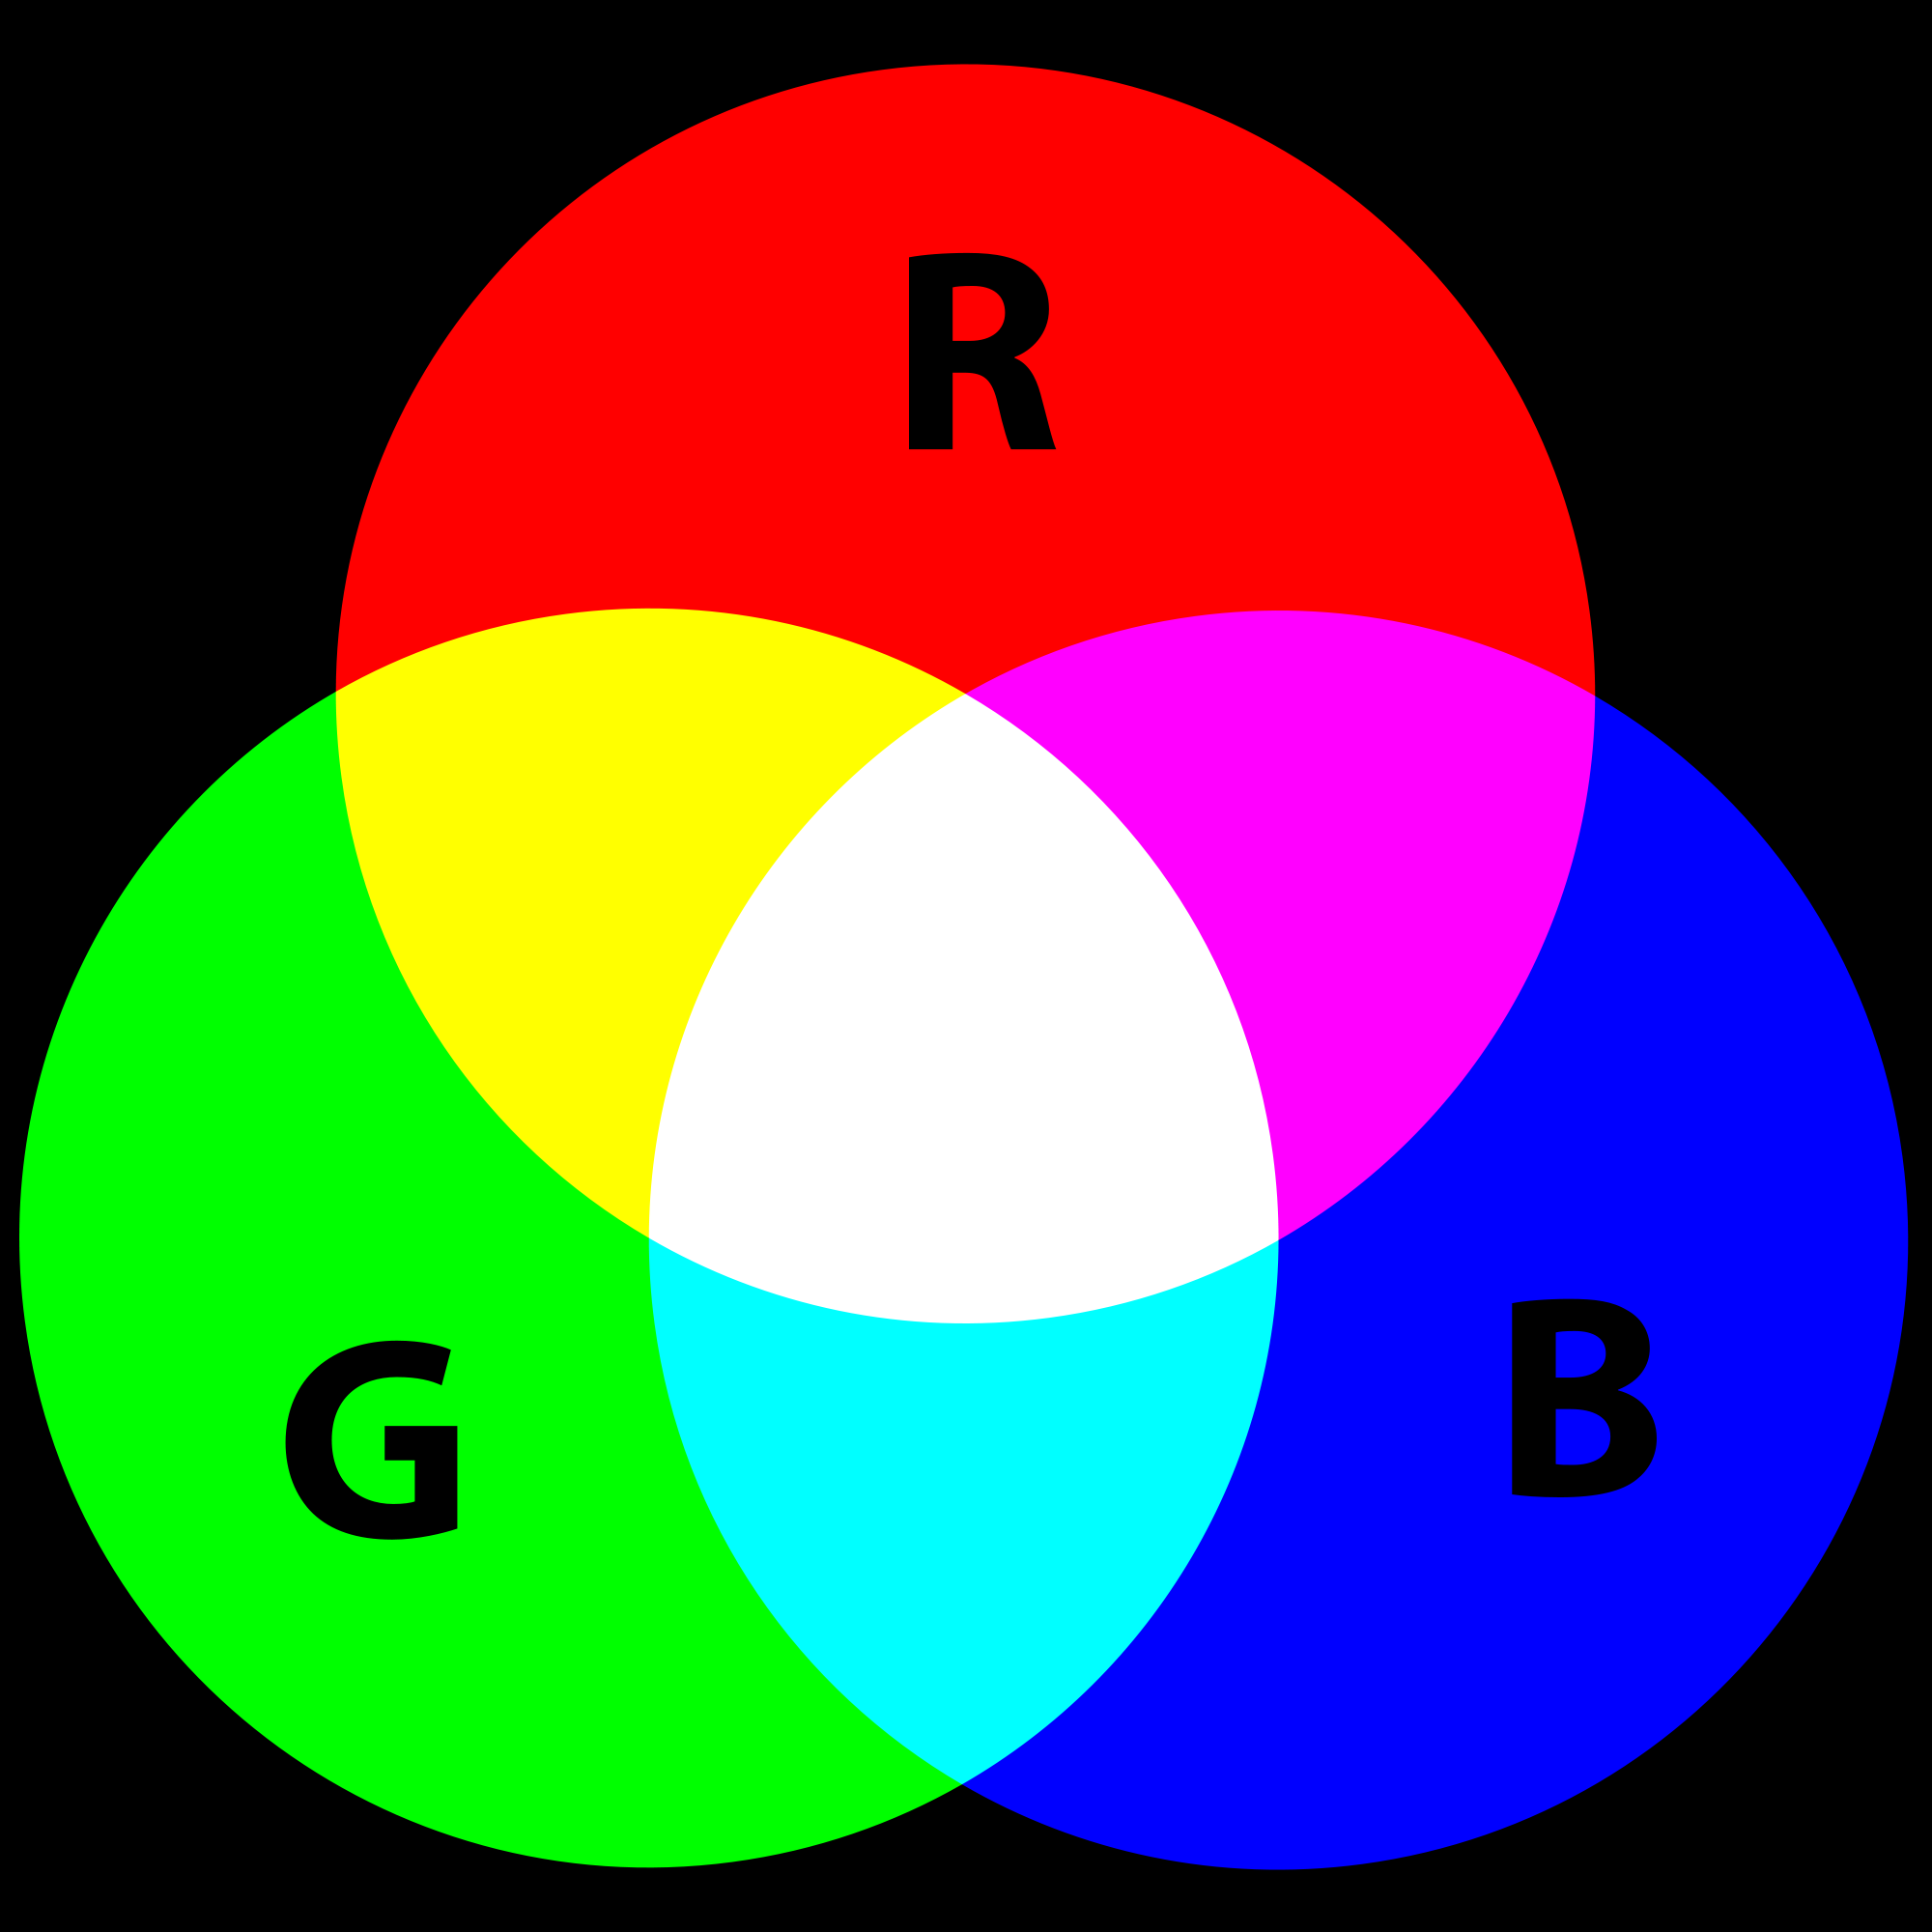
\includegraphics[width=0.4\textwidth]{img/RGB.png}
	\caption{RGB} 
	\label{fig:rgb}
\end{figure}

\subsubsection{HEX}
Hexadecimal represetation allows to write 3 RGB values as a single value,
followed by \# sign. Conversion can be done in two ways, which give equal
results:
\begin{enumerate}
  \item $HEX=R*256^2+G*256+B$,
  \item writing RGB values as three (two-digits long, from $00$ to $FF$)
  hexadecimal numbers, and writing them next to each other.
\end{enumerate}
Second way is much easier for humans because of lower values (3 values in
range 0-255, instead of one value up to about 16M). Also reverse operation
is much easier, because it requires only splitting of a string and changing
three low values from hex to decimal, instead of many divisions and modulo
operations. Some examples of hex values are:
\begin{itemize}
  \item $(0, 0, 0) \Leftrightarrow \#000000$,
  \item $(255, 255, 255) \Leftrightarrow \#FFFFFF$,
  \item $(0, 255, 0) \Leftrightarrow \#00FF00$,
  \item $(192, 192, 192) \Leftrightarrow \#C0C0C0$.
\end{itemize}

\subsection{Grayscale}
Grayscale is color system, which describes only intensity of color using a
single value (percentage, 0-1 or 0-255). Therefore after conversion to
grayscale, information about colors will be lost, and converting back will
result in also gray image, but described using RGB, with all values being equal.
This system is used mainly when there is no information about color, color is
not important, and/or for printing with only black ink.
\subsubsection{Conversion}
Conversion from RGB to grayscale can be done by calculating average value of RGB
values, and conversion in another direction by assigning one grayscale value to
all RGB ones.

\subsubsection{Examples}
Some examples for conversion between 0-255 RGB and 0-255 grayscale:
\begin{itemize}
  \item $(255, 0, 0) \Rightarrow 85 \Rightarrow (85, 85, 85)$
  \item $(0, 0, 255) \Rightarrow 85 \Rightarrow (85, 85, 85)$
  \item $(0, 127, 255) \Rightarrow 127 \Rightarrow (127, 127, 127)$
\end{itemize}
As it can be seen, this is a lossy conversion.

\subsection{HSV}
HSV (\textbf{H}ue, \textbf{S}aturation, \textbf{V}alue), is a color system
created to make choosing a color easier for humans. Instead of mixing three
values, person have to choose hue (color, shade), and then adjust its saturation
and value (brightness/lightness). HSV can be represented as cylinder, or as a
cone (fig. \ref{fig:hsv}). When looking from above, H is a degree on a wheel,
saturation is a distance from center (percentage of radius), and
value is deepth (percentage of cone/cylinder height).

\begin{figure}[!htb]
	\centering
	\includegraphics[width=0.5\textwidth]{img/hsv.png} 
	\caption{HSV cone}
	\label{fig:hsv}
\end{figure}

\subsubsection{Conversion from RGB}
Conversion from 0-255 RGB values can be done by formula:
\begin{equation}
\begin{split}
(R', G', B')&=(R, G, B)/255\\
C_{max}&=max(R', G', B')\\
C_{min}&=min(R', G', B')\\
\Delta&=C_{max}-C_{min}\\
\\
H&=\begin{cases}
0 & \Delta=0 \\
60\degree*(\frac{G'-B'}{\Delta}mod6) & C_{max}=R' \\
60\degree*(\frac{B'-R'}{\Delta}+2) & C_{max}=G' \\
60\degree*(\frac{R'-G'}{\Delta}+4) & C_{max}=B'
\end{cases} \\
S&=\begin{cases}
0 & C_{max}=0 \\
\frac{\Delta}{C_{max}} & C_{max} \neq 0
\end{cases}\\
V&=C_{max}
\end{split}
\end{equation}

\subsubsection{Conversion to RGB}
Conversion to 0-255 RGB values can be done by formula:
\begin{equation}
\begin{split}
C&=V*S\\
X&=C*(1-|H/60\degree|mod2-1)\\
m&=V-C\\
\\
(R', G', B')&=\begin{cases}
(C, X, 0) & 0\degree\leq H < 60\degree\\
(X, C, 0) & 60\degree\leq H < 120\degree\\
(0, C, X) & 120\degree\leq H<180\degree\\
(0, X, C) & 180\degree\leq H<240\degree\\
(X, 0, C) & 240\degree\leq H<300\degree\\
(C, 0, X) & 300\degree\leq H<360\degree
\end{cases}\\
\\
(R, G, B)&=((R'+m)*255, (G'+m)*255, (B'+m)*255)
\end{split}
\end{equation}

\subsubsection{Examples}
Some examples for conversion between 0-255 RGB and HSV:
\begin{itemize}
  \item $(0, 0, 0) \Leftrightarrow (0\degree, 0\%, 0\%)$,
  \item $(255, 255, 255) \Leftrightarrow (0\degree, 0\%, 100\%)$,
  \item $(255, 0, 0) \Leftrightarrow (0\degree, 100\%, 100\%)$,
  \item $(0, 255, 255) \Leftrightarrow (180\degree, 100\%, 100\%)$,
  \item $(128, 0, 128) \Leftrightarrow (300\degree, 100\%, 50\%)$.
\end{itemize}

\subsection{CMYK}
CMYK (\textbf{C}yan, \textbf{M}agenta, \textbf{Y}ellow,
Blac\textbf{k}/\textbf{K}ey value) is a substractive color model used mainly for
printing. In opposite for RGB (additive), where adding all colours results in
white color, in CMYK it gives black. It is so, because instead of adding light
sources, filters (e.g. paint), which remove colors, are added. Base color is
white (mix of all wavelenghts), and then filters are added, and only not
substracted colors are visible:
\begin{itemize}
  \item magenta substracts green,
  \item yellow substracts blue,
  \item cyan substracts red.
\end{itemize}
Therefore to obtain RGB base value, two CMY base values need to be used. It can
be seen on fig. \ref{fig:cmyk}. CMY colors can be also seen on fig.
\ref{fig:rgb} in RGB section. Black component (K) is added to CMY, because in
print, mixing all colors doesn't result in ideal black, and it is also cheaper
than using three colors. CMYK values are represented by four values, each for
intensity of one of colors. It can be percentage, 0-1 number, or 0-255 number.

\begin{figure}[!htb]
	\centering
	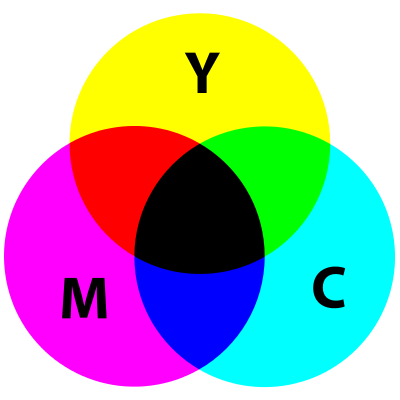
\includegraphics[width=0.4\textwidth]{img/CMYK.png}
	\caption{CMYK} 
	\label{fig:cmyk}
\end{figure}

\subsubsection{Conversion from RGB}
Conversion from 0-255 RGB values to 0-1 CMYK can be done by formula:
\begin{equation}
\begin{split}
(R', G', B') &= (R, G, B)/255 \\
K&=1-max(R', G', B')\\
C&=(1-R'-K)/(1-K)\\
M&=(1-G'-K)/(1-K)\\
Y&=(1-B'-K)/(1-K)
\end{split}
\end{equation}
\subsubsection{Conversion to RGB}
Conversion to 0-255 RGB values from 0-1 CMYK can be done by formula:
\begin{equation}
\begin{split}
R&=255*(1-C)*(1-K)\\
G&=255*(1-M)*(1-K)\\
B&=255*(1-Y)*(1-K)
\end{split}
\end{equation}

\subsubsection{Examples}
Some examples for conversion between 0-255 RGB and CMYK:
\begin{itemize}
  \item $(0, 0, 0) \Leftrightarrow (0, 0, 0, 1)$,
  \item $(255, 255, 255) \Leftrightarrow (0, 0, 0, 0)$,
  \item $(255, 0, 0) \Leftrightarrow (0, 1, 1, 0)$,
  \item $(0, 255, 0) \Leftrightarrow (1, 0, 1, 0)$,
  \item $(0, 255, 255) \Leftrightarrow (1, 0, 0, 0)$.
\end{itemize}

\section{Used technologies}
Project was written in pure Java 8 using only build-in datatypes and functions, including Java's standard GUI library Swing using integrated development environment Eclipse Mars.
The conversion algorithms were written by us, with implementation similar to build-in ones and checked for correctess with our owrn Java standard testing framework JUnit.
Git and trello were used to help in management of the project.

\clearpage
\section{Application Functionality}
The application provides user with an intuitive graphical interface. On the left
side there is a color conversion panel (Figure~\ref{fig:conv}), that provides
automatic translation between RGB, RGB written as hex word, CMYK, Grayscale and
HSV systems. Each of those fields is editable and as long as the data is valid,
an automatic conversion will take place and all other field's values will be
updated. There is also a large rectangle representing the choosen color.

\begin{figure}[!htb]
	\centering
	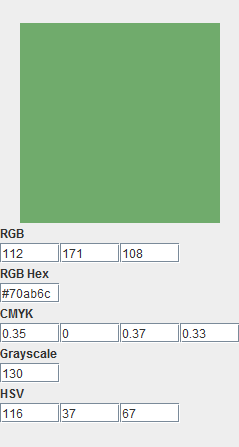
\includegraphics[width=0.35\textwidth]{img/conversion.png} 
	\caption{Color conversion panel}
	\label{fig:conv}
\end{figure}

On the right side one of three tabs can be selected. Image picker lets the user
select a pixel from a loaded image, filling the conversion panel with its value
in all available systems.

\begin{figure}[!htb]
	\centering
	
\includegraphics[width=0.4\textwidth]{img/imagepick.png}
	\caption{Picking color from image} 
	\label{fig:image}
\end{figure}

Another tab, HSV Picker, lets the user choose a color using a two dimensional
representation of a HSV cone. Slider at the top is linked to the Hue and using
it changes the crossection showed as a triangle beneath. Clicking on a color on
this triangle updates the color conversion panel with the colors values in
available systems. HSV cone enables easy access to similar colors for the user.

\clearpage
\begin{figure}[!htb]
	\centering
	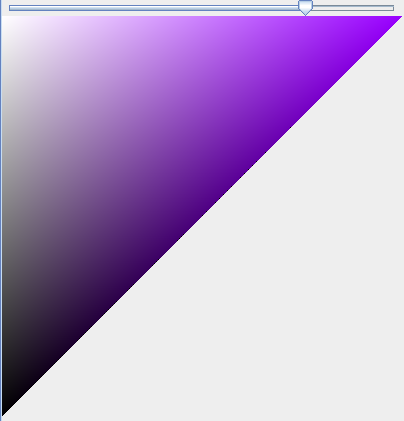
\includegraphics[width=0.5\textwidth]{img/hsvpick.png} 
	\caption{Picking color from HSV cone}
	\label{fig:hsv_pick}
\end{figure}

Next tab, called RGB picker, consists of three sliders with a colourful strip
under each one. Each slider represents the value of red, green or blue part of
the RGB color scheme respectively. Each strip represents the colors that are
available when changing just the value of the connected slider. Each change in
the sliders will update conversion panel with the selected color. Additionally
each change in the conversion panel will change the picked in this component.

\begin{figure}[!htb]
	\centering
	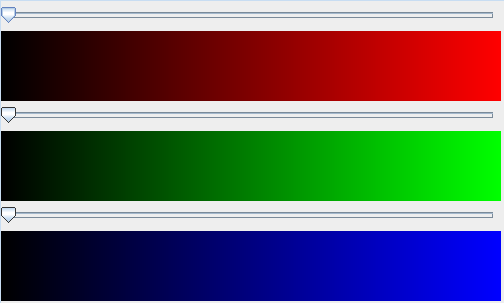
\includegraphics[width=0.7\textwidth]{img/rgbpick.png} 
	\caption{Picking color from RGB sliders}
	\label{fig:rgb_slider}
\end{figure}

% TODO Conclusions - potrzebujemy?
\end{document}